% 天文学常识

\subsection{太阳系模型}

\begin{figure}[ht]
\centering
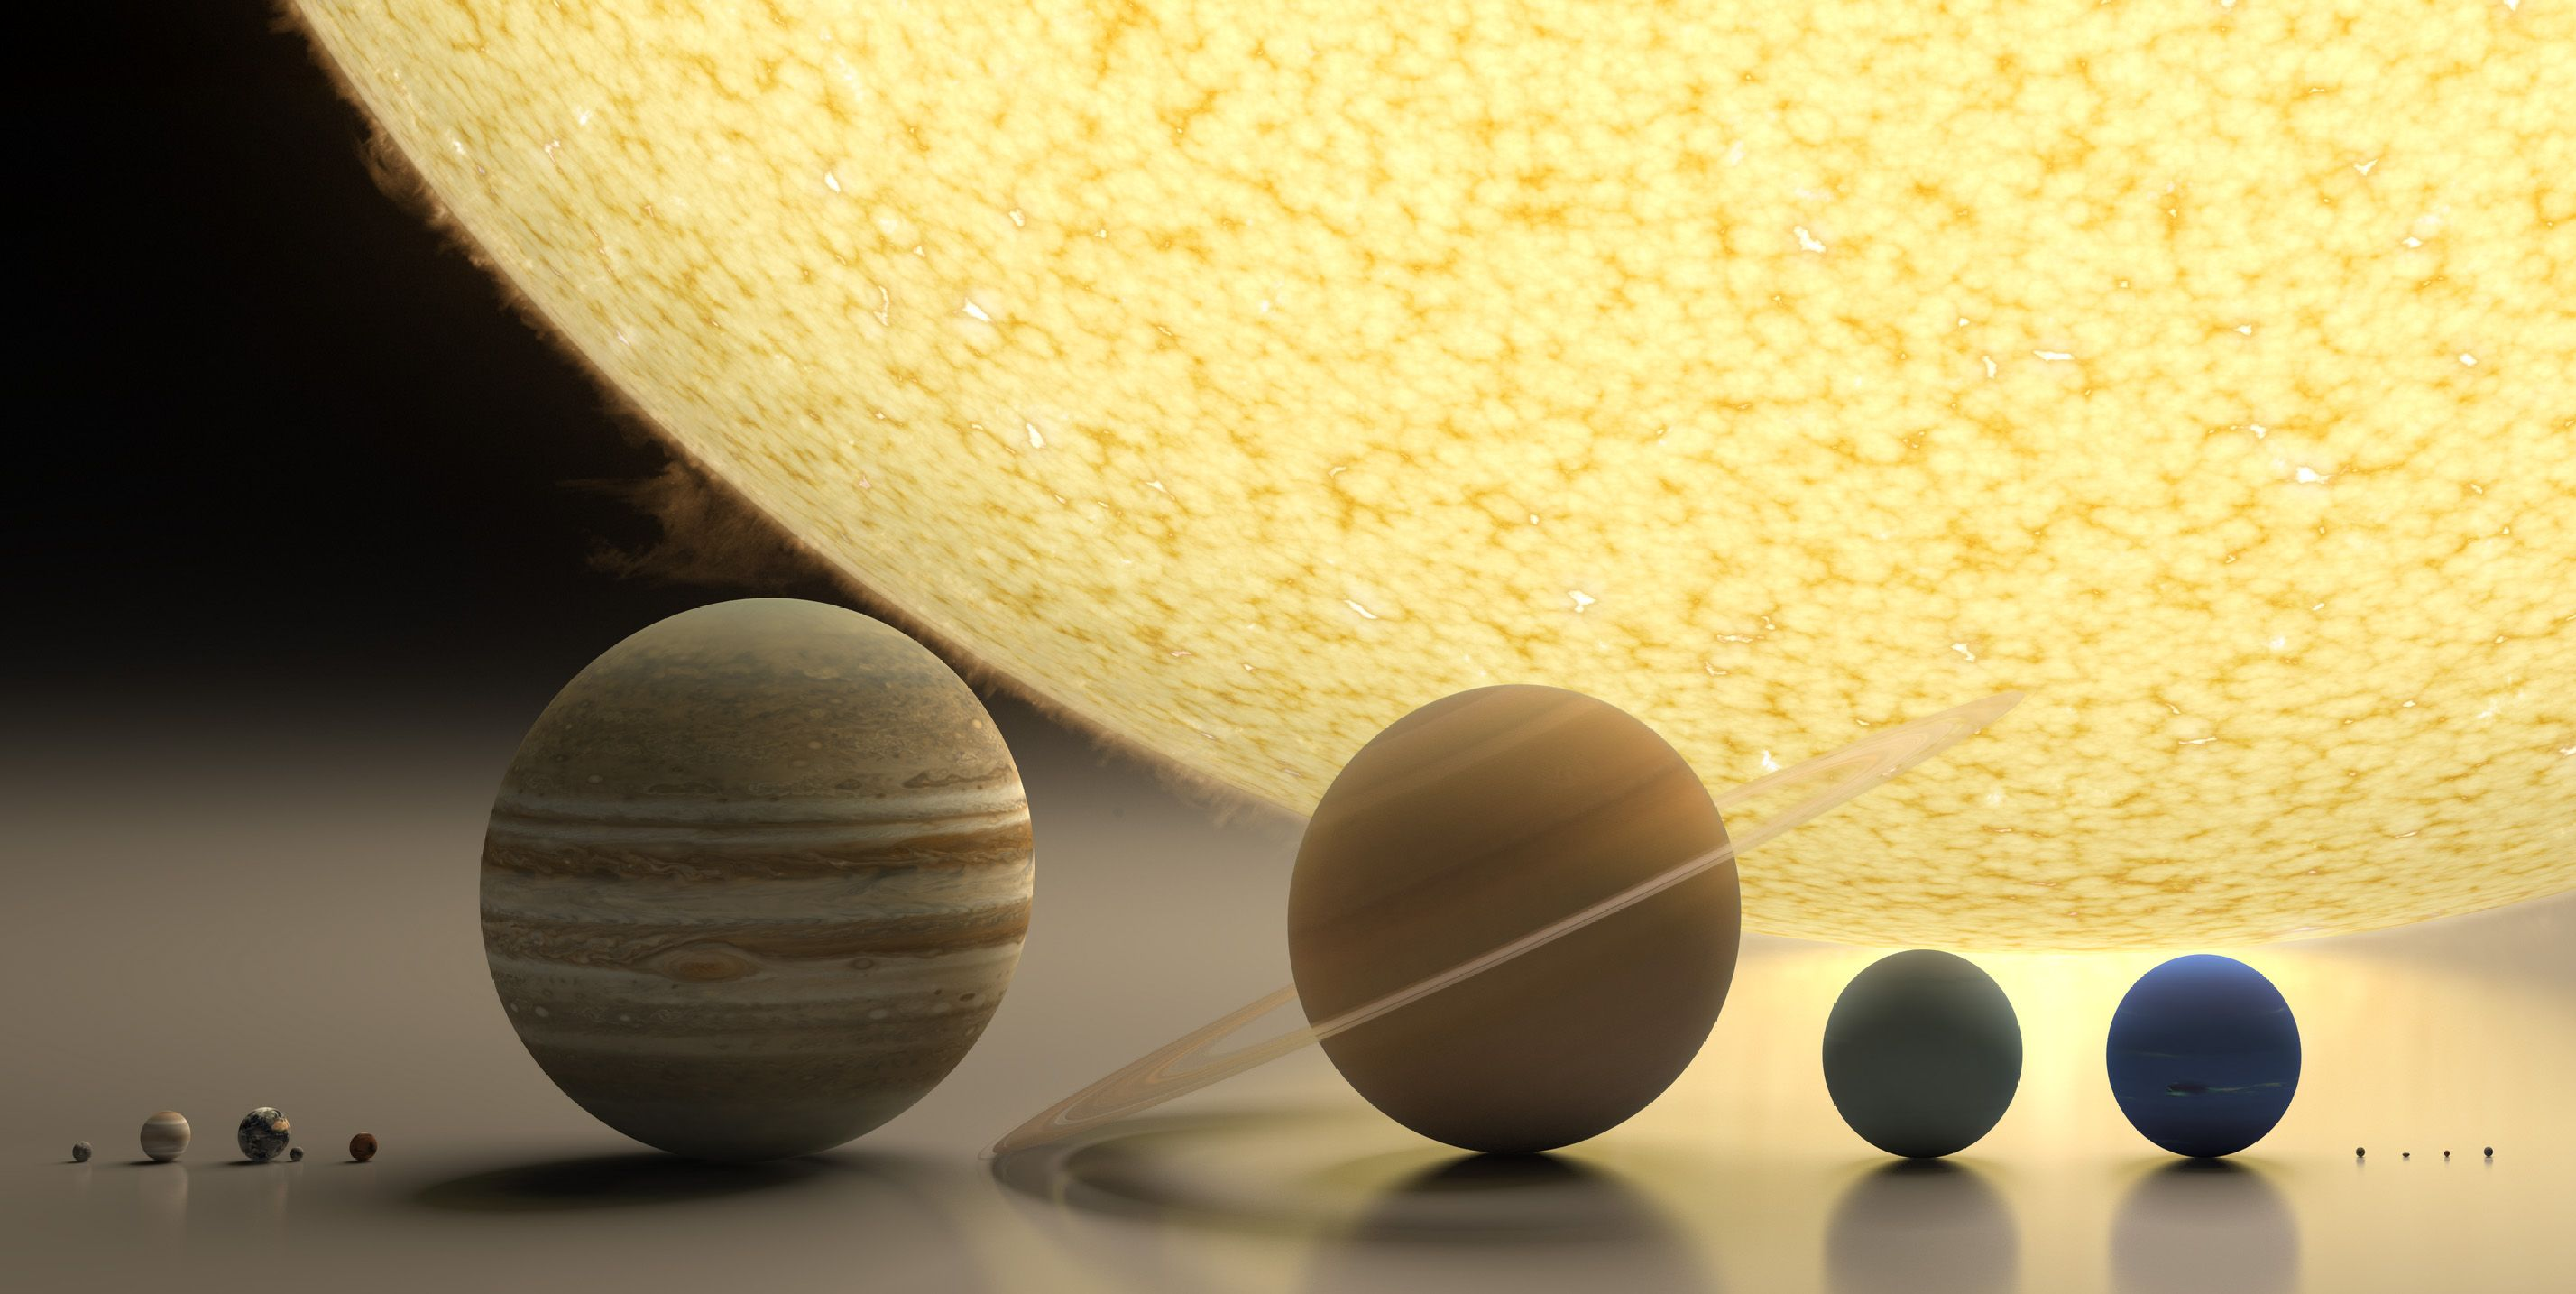
\includegraphics[width=14cm]{./figures/Astro1.pdf}
\caption{真实比例下太阳与行星的大小(来自 pinterest.com), 行星从左到右依次为水星, 金星, 地球(及月亮), 火星, 木星, 土星, 天王星, 海王星, 其他小行星} \label{Astro_fig1}
\end{figure}

恒星和行星一个显著的区别就是恒星很大, 而且会发光。 太阳是太阳系中唯一一个恒星, 其他天体都不发光, 而是反射太阳的光。

首先一个误区就是行星的尺寸和距离, 大部分太阳系模型的比例都是完全错误的, 原因是如果按照真实比例制作模型, 要么就是行星小得看不到, 要么就是模型大得不切实际。 我们这里来构建一个符合比例的太阳系模型, 即用乒乓球来代表太阳, 再按比例计算其他长度和距离, 结果见\autoref{Sample_tab1}。

\begin{table}[ht]
\centering
\caption{太阳系的一些数据}\label{Sample_tab1}
\begin{tabular}{|c|c|c|}
\hline
 & 真实长度 & 模型长度 \\
\hline
太阳半径 & $6.96\times 10^5 \Si{km}$ & $20\Si{mm}$\\
\hline
地球半径 &  $6.37\times 10^3 \Si{km}$ & $0.183 \Si{mm}$\\
\hline
地球到太阳  &  $1.46 \times 10^8 \Si{km}$ & $22.4 \Si{m}$\\
\hline
月球半径 & $1.74 \times 10^3 \Si{km}$ & $0.05 \Si{mm}$\\
\hline
月球到地球 & $3.84 \times 10^5 \Si{km}$ &  $1.10 \Si{cm}$\\
\hline
土星半径 & $7.15 \times 10^4 \Si{km}$ & $2.05 \Si{mm}$\\
\hline
土星到太阳 & $7.79 \times 10^8 \Si{km}$ & $22.4 \Si{m}$\\
\hline
冥王星到太阳 & $5.91 \times 10^9 \Si{km}$ & $128 \Si{m}$\\
\hline
最近的恒星到太阳 & $3.99 \times 10^{13} \Si{km}$ &  $1147 \Si{km}$\\
\hline
\end{tabular}
\end{table}

\subsection{星空}

\begin{figure}[ht]
\centering
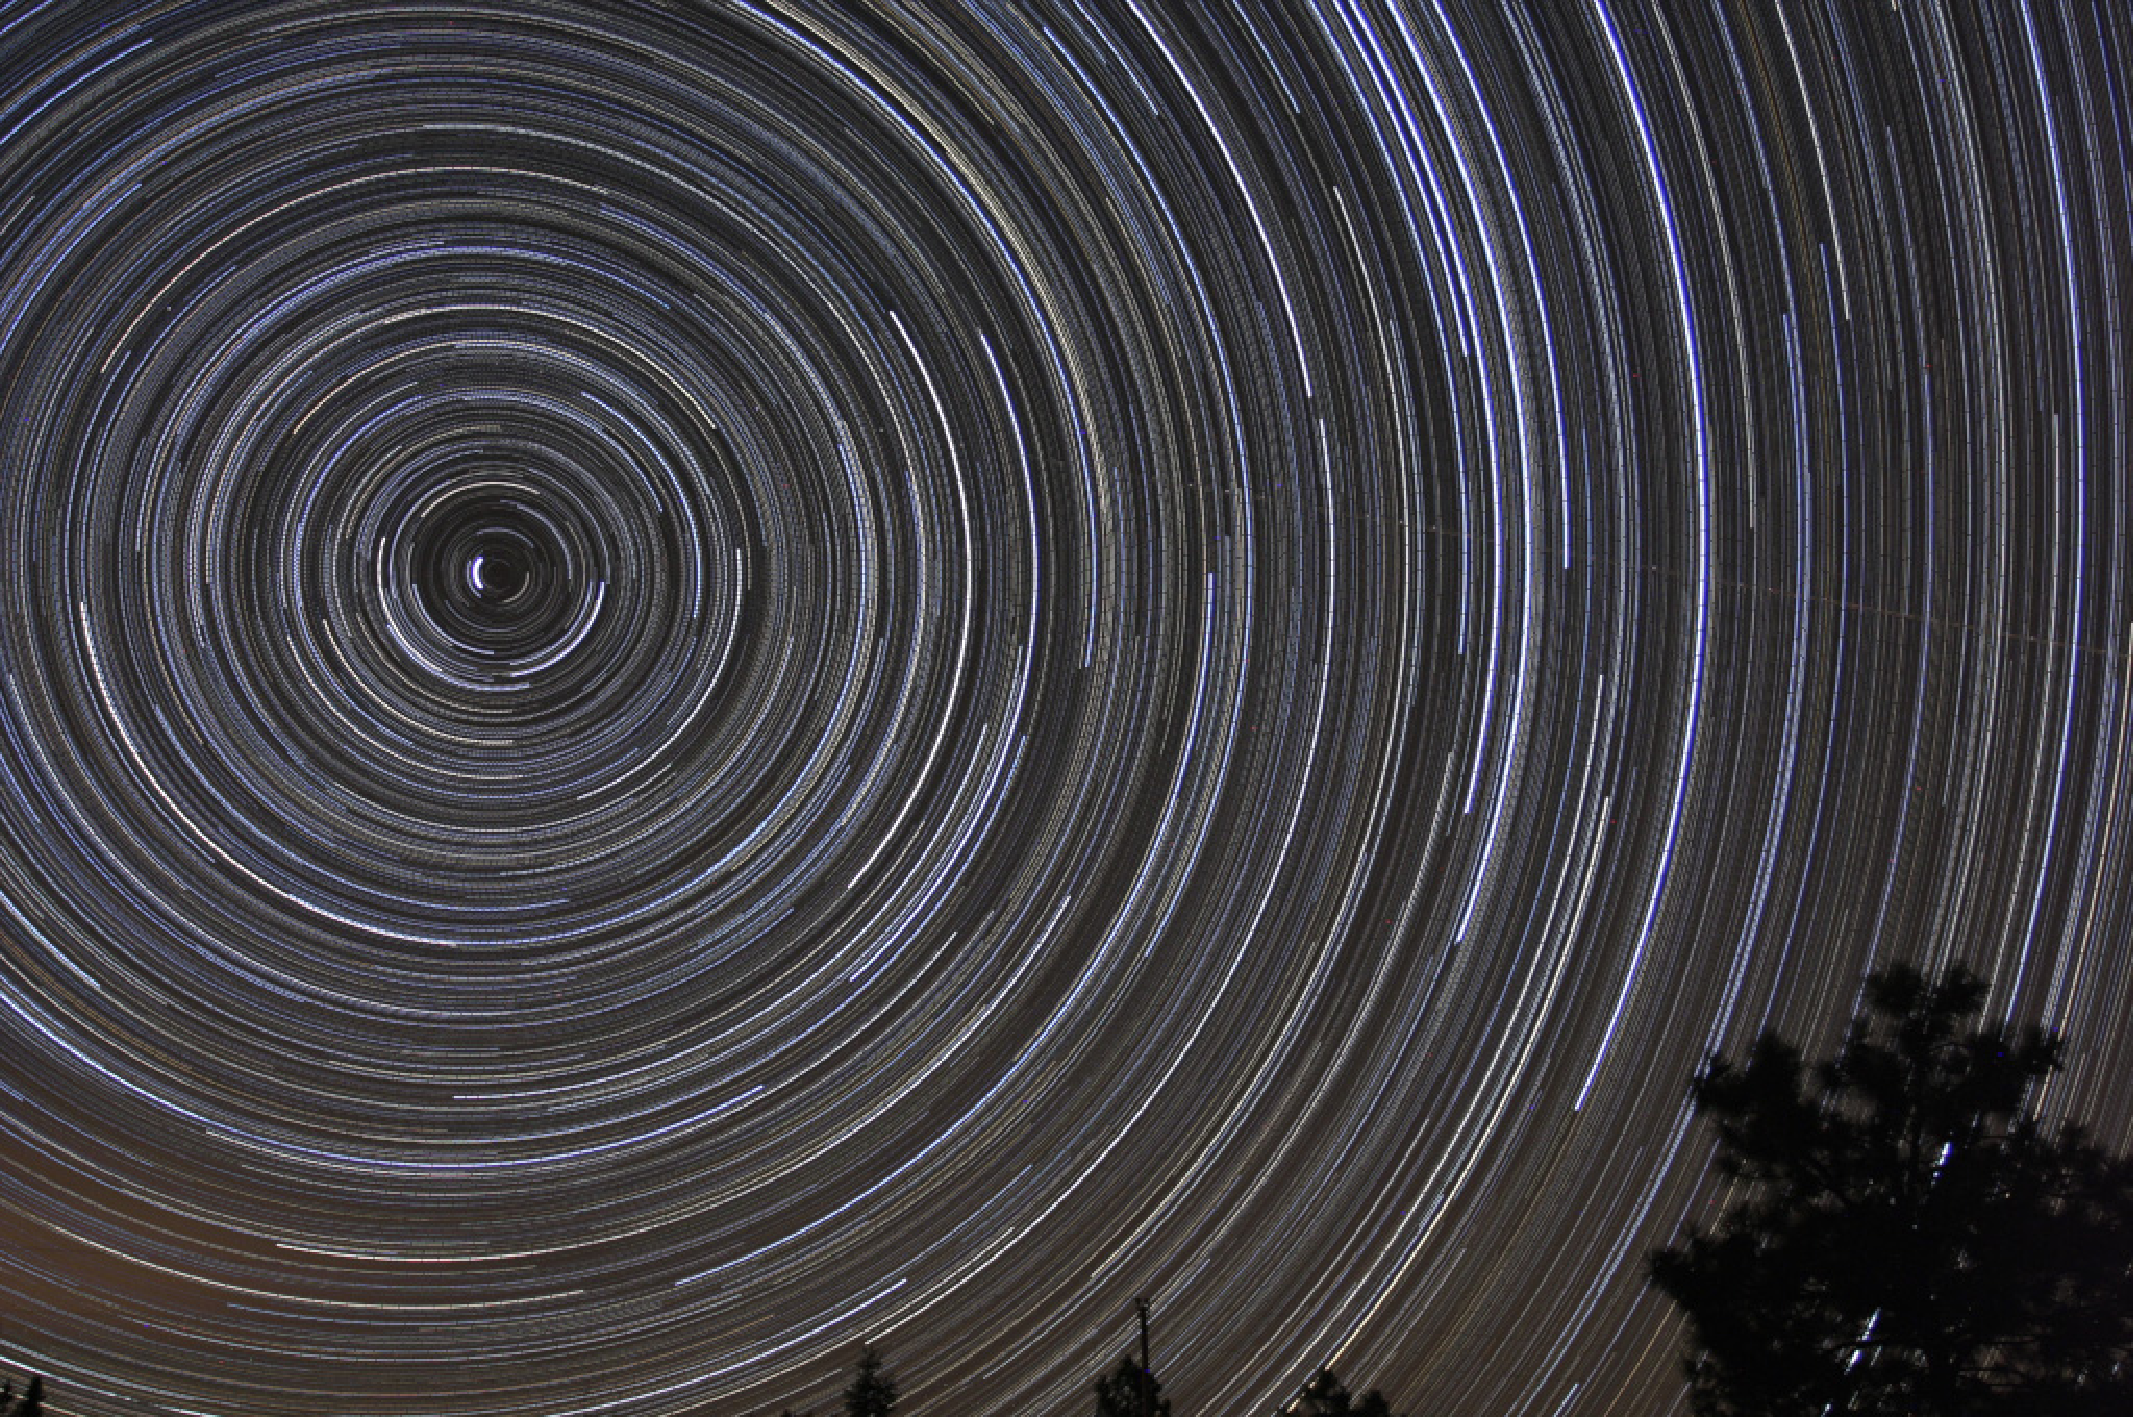
\includegraphics[width=14cm]{./figures/Astro2.pdf}
\caption{星星的轨迹(来自 burro.case.edu), 注意如果测量图中每条弧线的张角就可以计算曝光的时间} \label{Astro_fig2}
\end{figure}

除了太阳系中的天体, 肉眼或望远镜能看到的其他星星都属于恒星(注意有一些亮点是星云, 即星际尘埃而不是单个恒星), 离太阳最近的恒星叫做 Alpha Centauri (4.22 光年)。 由于这些恒星的距离太远, 即使用天文望远镜也看不到它们的行星。 恒星在空中的相对位置是几乎不变的(即使太阳系以惊人的速度绕星系中心旋转, 但转一圈仍需要 2.3 亿年, 所以与其他恒星的相对位置基本保持不变)。

那我们看到的星空是如何变化的呢? 由于地球每 24 小时由西向东自转一圈, 所以我们在地球上看到的星空由东向西围绕地球旋转。 长时间曝光的照片可以很好地展示星星的轨迹(\autoref{Astro_fig2})。 如果站在北极点, 那么星空的旋转中心会在正上方, 如果站在赤道, 旋转中心会在地平线上, 且南北各有一个。 如果站在南极点, 则旋转中心同样在正上方但旋转方向却与北极的相反。

一个常见的问题是为什么白天看不到星星和月亮。 这是因为白天阳光照亮了大气中的尘埃和云, 相比之下星星的亮度太暗了所以肉眼不容易看到。 许多时候月亮也会在白天出现在太阳附近, 也是因为阳光不容易注意到。

下面我们来更具体地描述星空, 如(图未完成)所示, 我们可以想象地球处于一个比地球大得多的玻璃球中心, 所有的星星都画在玻璃球上, 且随玻璃球旋转。 现在如果观察者站在某个纬度观测星空, 他看到的玻璃球将会是这样的(图未完成)。



\subsection{昼夜}

% 未完成: 说明日长与纬度的关系, 极昼和极夜, 



而地球自转的转轴却并不垂直于该平面, 而是有约 23.5° 的倾角。



地球 24 小时自转一周, 在这段时间内, 地球和太阳的相对位置可以近似认为不变。 如果我们能同时看到太阳和行星, 太阳在星空背景上的位置也近似不变。 而上文描述了星空如何围绕地球旋转, 你可以相像其中一个星星是太阳。



), 这在地球上看来就相当于太阳绕地球旋转。 由于太阳非常远, 达到地球的阳光几乎可以看成是平行的, 这样地球的一半就会被照亮, 这一半就是白天, 而另一半是黑夜。

地球绕太阳旋转轨道所在的平面叫\bb{黄道平面}, 我们不妨先想像地球自转的转轴垂直于该平面垂直。 












